%%% Results %%%
\chapter{Results} \label{ch:results}
 
\section{XY model on SAWs, 2D}
To perform MC simulations for short chains from $N=100$ to $N=1000$, we run at least $2.1 \times 10^9$ MC steps using two  types of updates: snake-like and reconnect. We choose following update probabilities: $P_{local}=0.8$, $P_{reconnect}=0.2$. 

For longer chains $N>1000$ we additionally use cluster update. For $N=4900$, we run at least $8 \times 10^{10} $ MC steps. Here we use these values for update probabilities: $P_{local}=0.8$, $P_{reconnect}=0.199$, $P_{Wolff}=0.001$.

 
\subsection{Tests for validation simulations}
To test our Monte-Carlo (M) simulation, we compare results obtained using MC and Sampling + Exact Enumeration (EE). This method is not reliable, but it helps to make approximate checks. For short chains ($N=5, N=8$), we generate all set of self-avoiding walks by EE and sample spin configurations by uniform distribution $U(-\pi, \pi)$. As this is resource-consuming procedure, we sample spin configurations only $600$ times (so, 600 sequences of spins applied to each conformation) and repeat this $10$ times. Figure \ref{fig:ee} shows obtained results.  For $J=0$, the second moment of magnetization are close to exact values \eqref{m2j0} and the mean energy starts at $\langle e \rangle = 0$.

 \begin{figure}[H]
	\centering
	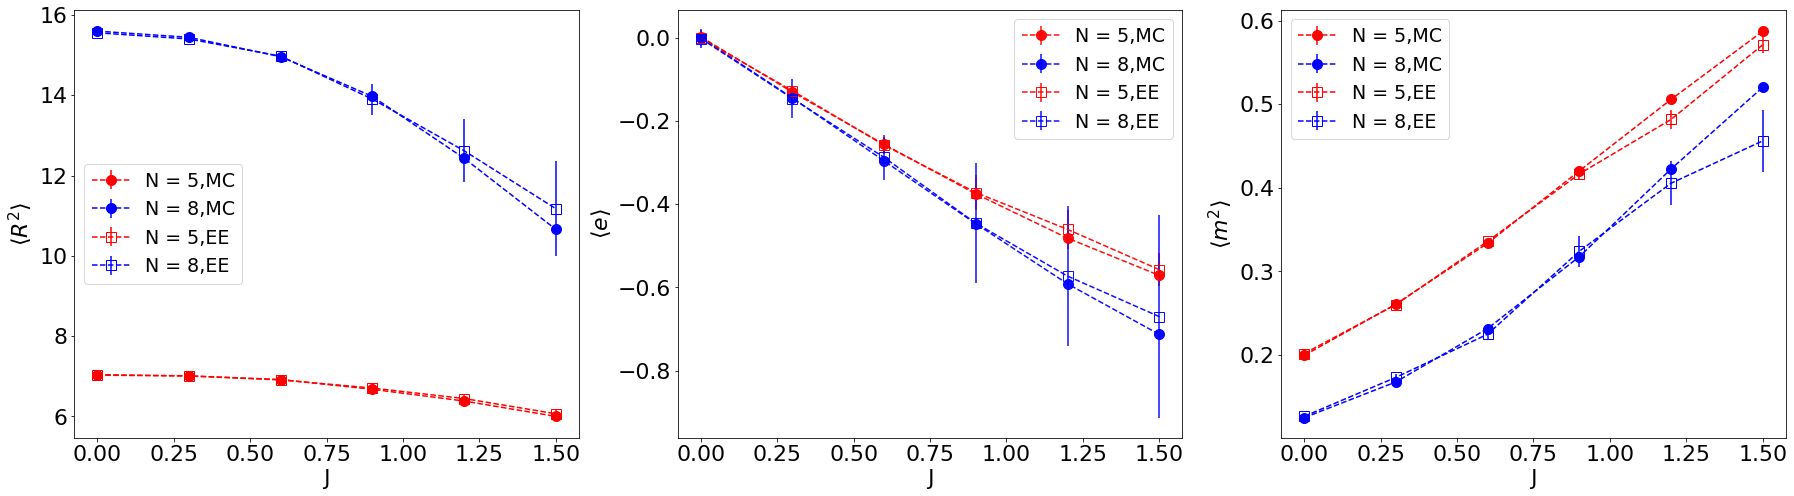
\includegraphics[scale=0.26]{Images/EE.png}
	\caption{$h=0$. Mean Radius \eqref{endtoend}, mean energy \eqref{hamiltonian} and   second moment of magnetization \eqref{secondmomentmagnetization}.   }
	\label{fig:ee}
\end{figure}


\subsection{Thermodynamic properties}
First, we measure the mean square magnetization \eqref{secondmomentmagnetization} and the mean energy \eqref{hamiltonian} for short chains (up to $N=1000$) in the large range of the interaction energy $J$ and for long chains (up to $N=4900$) in the narrow range where the system are expected to undergo the phase transition.

 \begin{figure}[t]
	\centering
	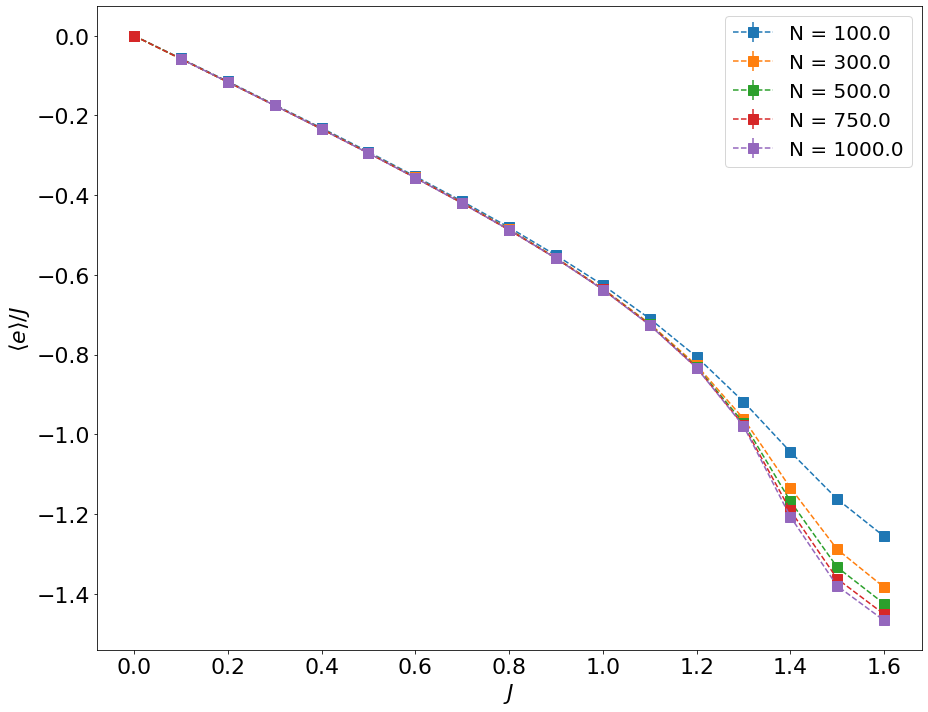
\includegraphics[scale=0.23]{Images/energy_shortchains.png}
	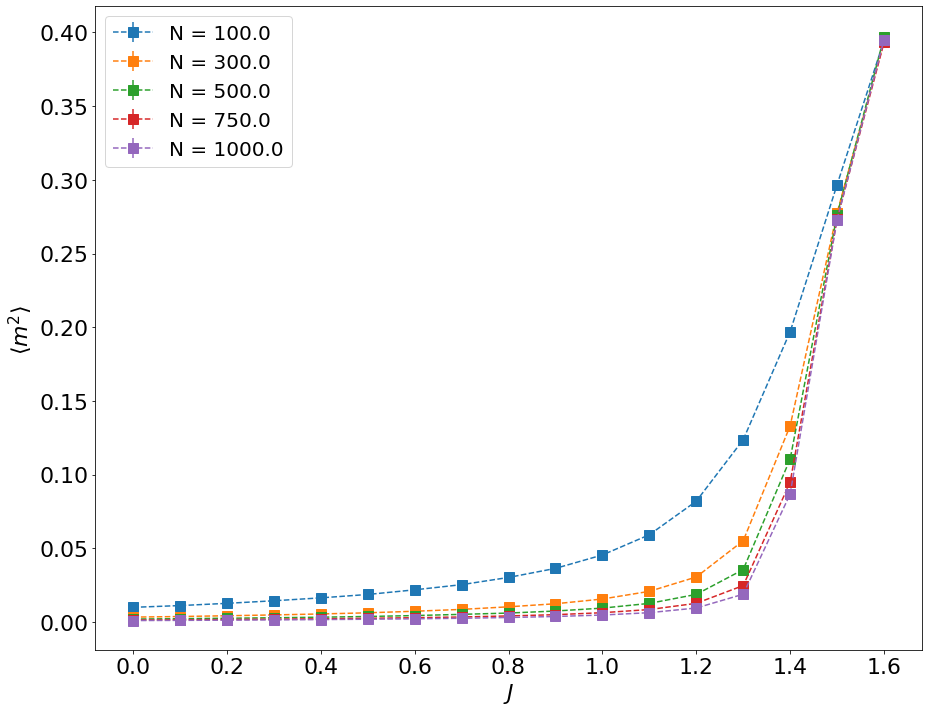
\includegraphics[scale=0.23]{Images/magnetization2_shortchains.png} \\
	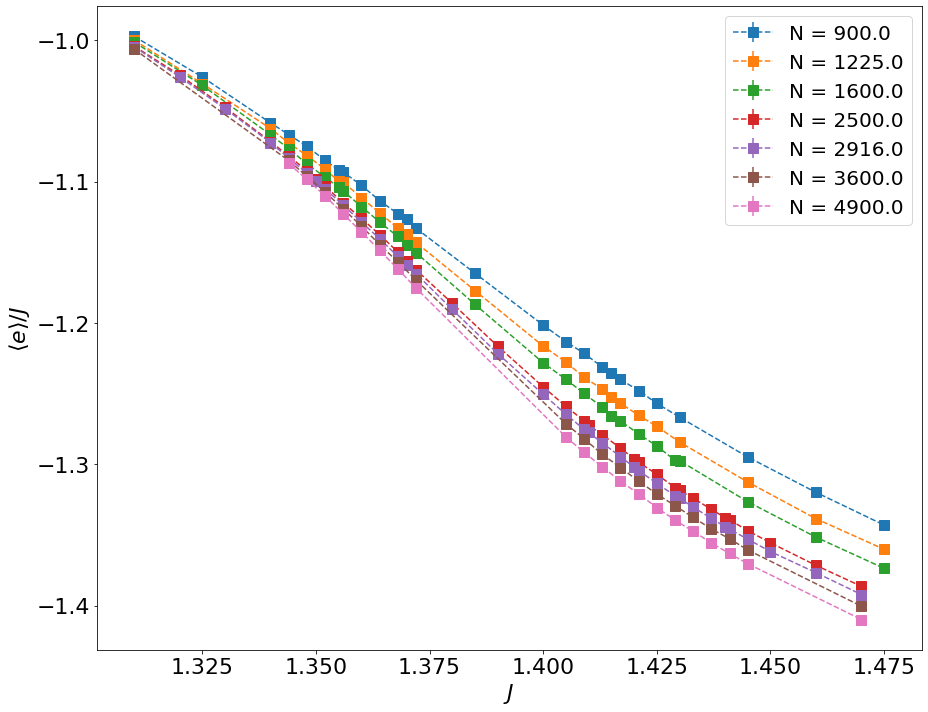
\includegraphics[scale=0.23]{Images/energy_longchains.png}
	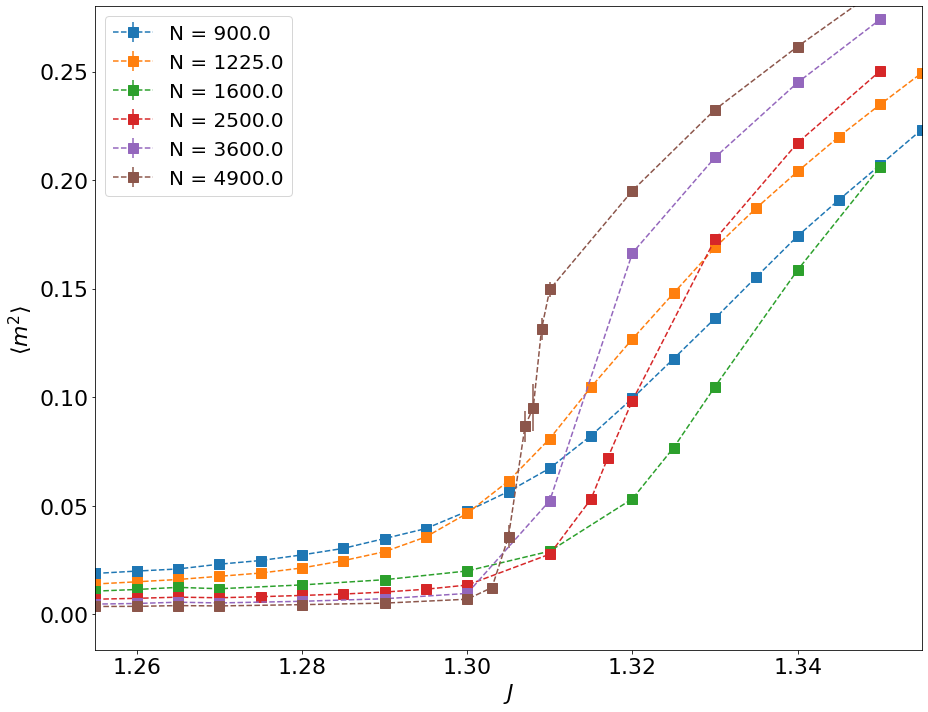
\includegraphics[scale=0.23]{Images/magnetization2_longchains.png}
	\caption{$h=0$. Mean energy \eqref{hamiltonian} and   second moment of magnetization \eqref{secondmomentmagnetization}. }
	\label{fig:energymagshort}
\end{figure}

 Figure \ref{fig:energymagshort} (left column) shows computational results for the mean energy  \eqref{hamiltonian} as a function of $J$. At the top plot for short chains, the mean energy starts at $\langle e \rangle = 0$ as expected for unfolded disordered SAWs. As $N \rightarrow \infty$, the value of the mean energy decreases and goes to the asymptotic value $\langle e \rangle = -2J$ for compact ordered walk. 
 
  Figure \ref{fig:energymagshort} (right column) illustrates obtained numerical results for the second moment of magnetization \eqref{secondmomentmagnetization}. At $J=0$, results are consisted with the exact solution \eqref{m2j0} and $  \langle m^2 \rangle  \rightarrow 0$ as $N \rightarrow \infty$. As $J$ increases, the square of magnetization grows up. One can suppose an ordering behavior for large J.
  
  From both energy and the second magnetization moment, we can clearly see the finite size effect. The longer chains has jumps in the function for lower $J$ in comparison to shorter ones. 
 
 
%Figure \ref{fig:energymagshort} illustrates obtained results for Mean energy \eqref{hamiltonian} and   second moment of magnetization \eqref{secondmomentmagnetization}. The system tends to order as interaction energy $J$ gets larger. 
\subsection{Structural properties}

Next, we estimate critical exponent $\nu$ \eqref{r_scale} from the asymptotic power law for the mean square end-to-end distance of SAWs. We use following ansatz  \cite{Berretti1985}:
\begin{equation}
\label{berettiscale}
\log (R_N^2+k_1 ) = 2 \nu \log (N+k_2) + b.
\end{equation}
Here $k_1=k_2=1$ are phenomenological parameters. 
 \begin{figure}[H]
	\centering
	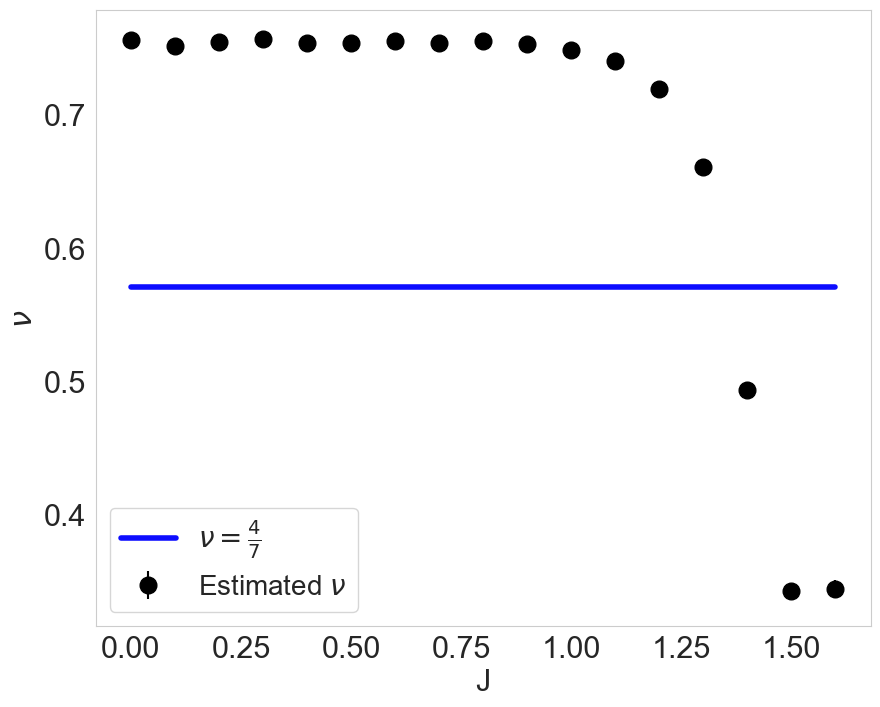
\includegraphics[scale=0.36]{Images/nu_shortchains.png}
	\caption{$h=0$. Estimations with errorbars of critical exponent $\nu$ .   }
	\label{fig:nushort}
\end{figure}
 

For the start, we perform curve-fitting for short chains on the large range of values $J$. Figure \ref{fig:nushort} illustrates obtained results of exponent estimation. In $J=0$, the critical exponent $\nu$ equals $\nu = \frac{3}{4}$  which is consisted with the value of non-interacting SAWs \eqref{nur}. The value $\nu=\frac{4}{7}$, which is the exact value
for interacting SAWs \eqref{nu_theta}, appears at the region $ 1.25 < J < 1.4$. In previous section we showed that the energy and second magnetization moment functions of $J$ have jumps approximately at the same region. 

  We can assume that XY model on SAWs also has value $\nu = 4/7$ \eqref{nu_theta} at the point of structural phase transition. We use this value to obtain collapsing plots in Figure \ref{fig:bcshort} in following subsection \ref{section:Transition}. 

%\section{Scalings}
%Next, we move to estimation of the crossover exponent $\phi$ which
%quantifies the deviation from criticality via the scaled coupling $x = (J-J_c) / N^{-\phi}$ \cite{van2015statistical}. In \cite{PhysRevE.104.024122, PhysRevE.104.054501} it was assumed the value $\phi \approx 0.71$. We use this value to produce scaling plots \ref{fig:radiusscaling}. 
%\begin{figure}[H]
%	\centering
%	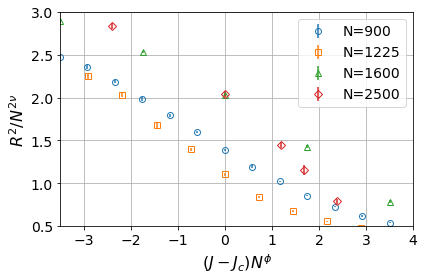
\includegraphics[scale=0.23]{Images/R2_data_collapse_phi.png} 	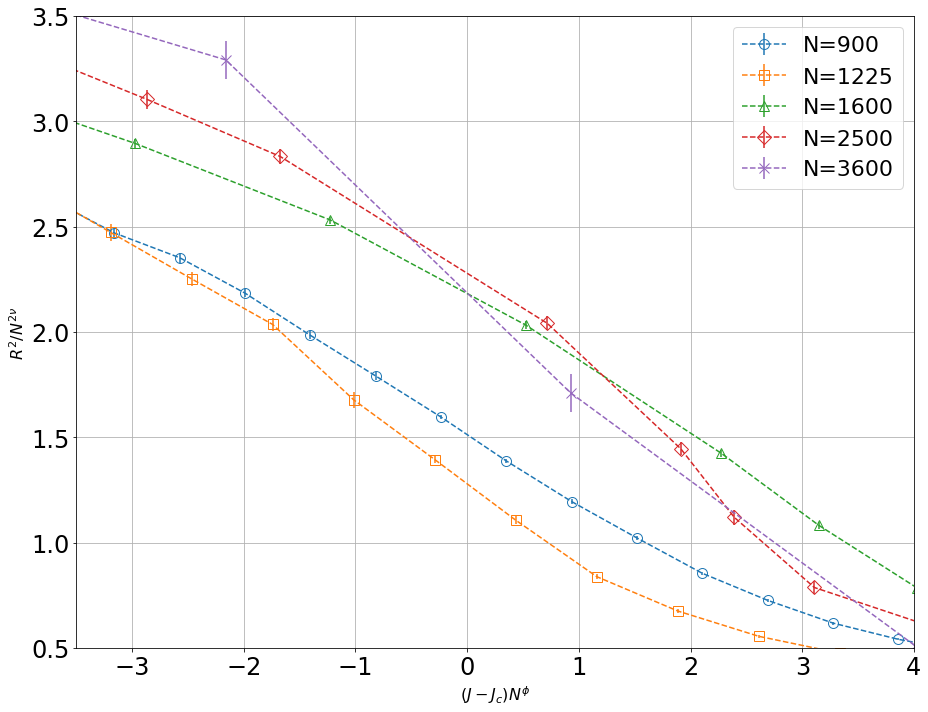
\includegraphics[scale=0.23]{Images/R2_data_collapse_phi1.png} \\ 
%	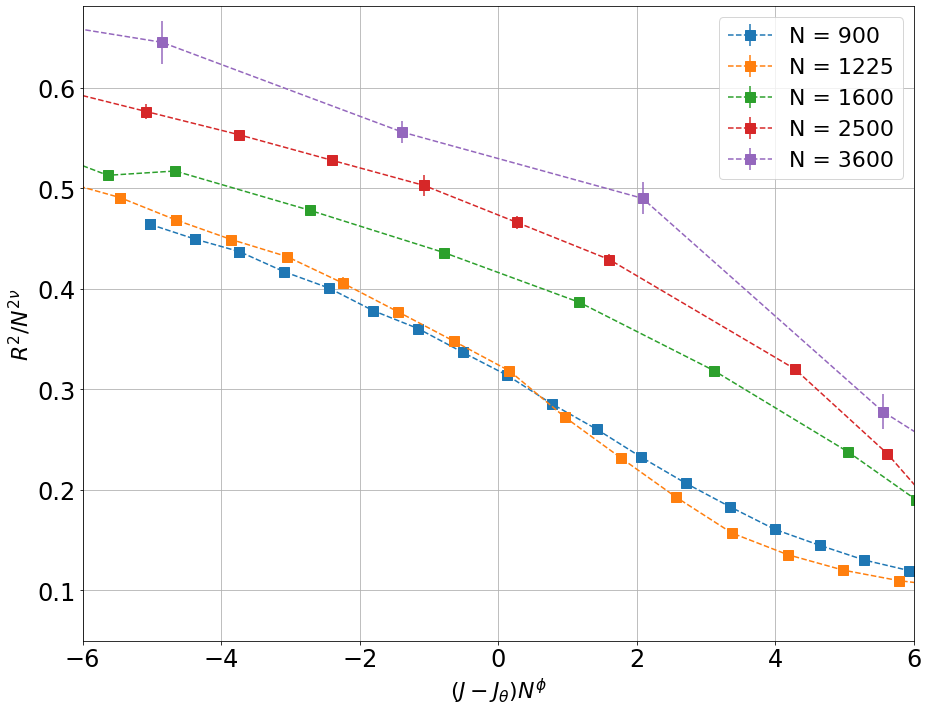
\includegraphics[scale=0.23]{Images/rscalinglong_dc.png}
%	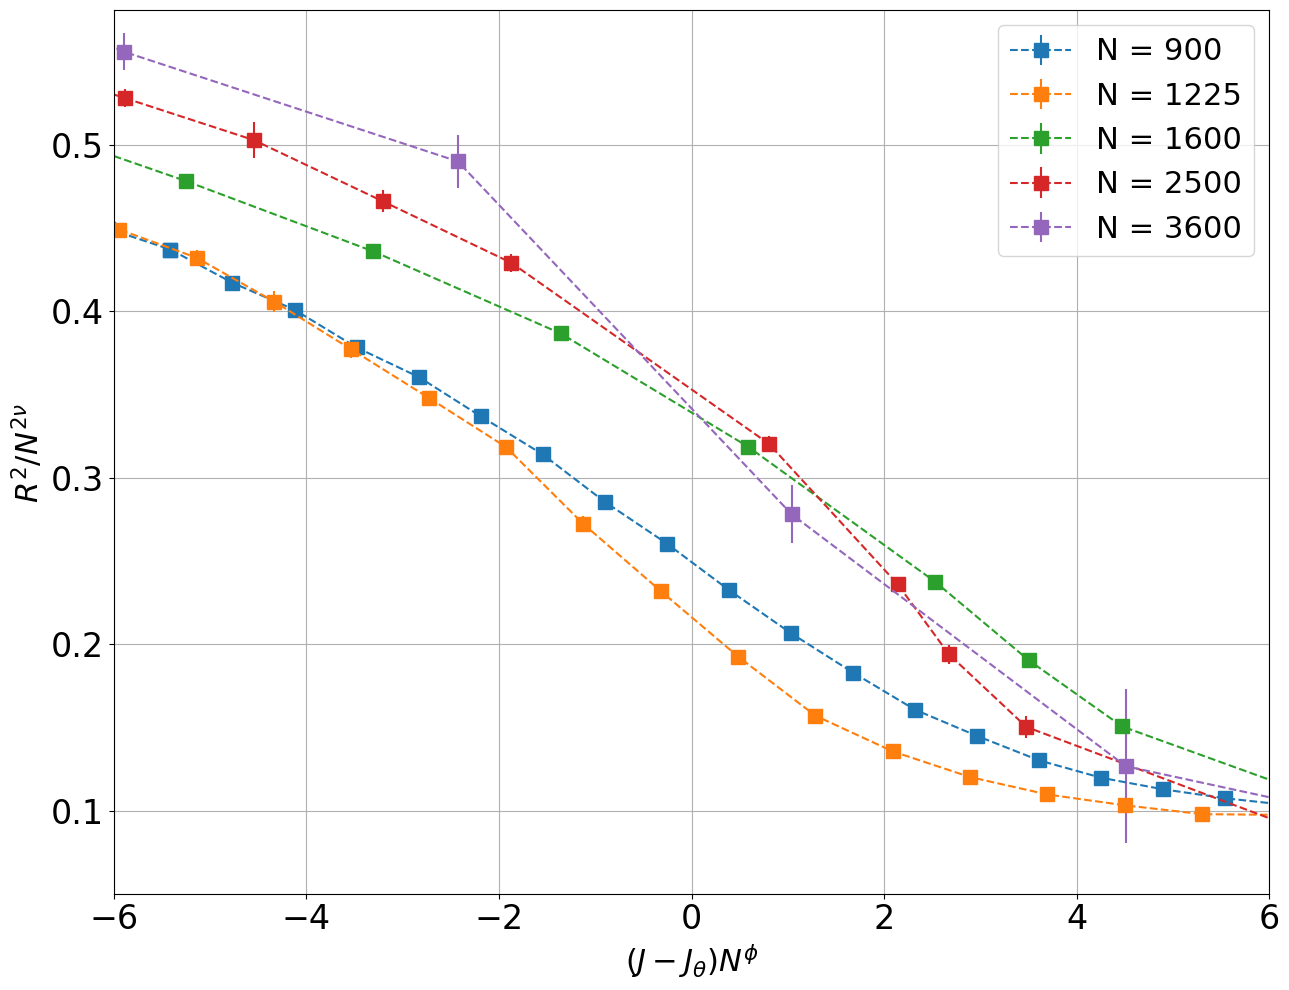
\includegraphics[scale=0.23]{Images/rscalinglong_dc1.png} 	\\
%		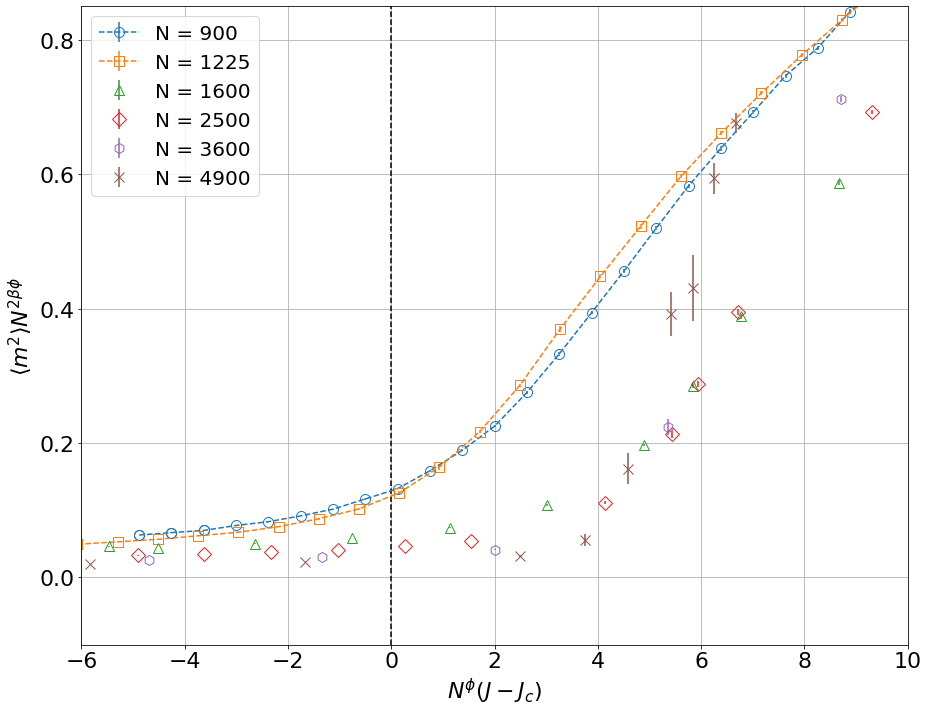
\includegraphics[scale=0.23]{Images/2dmag2scaling.png} 	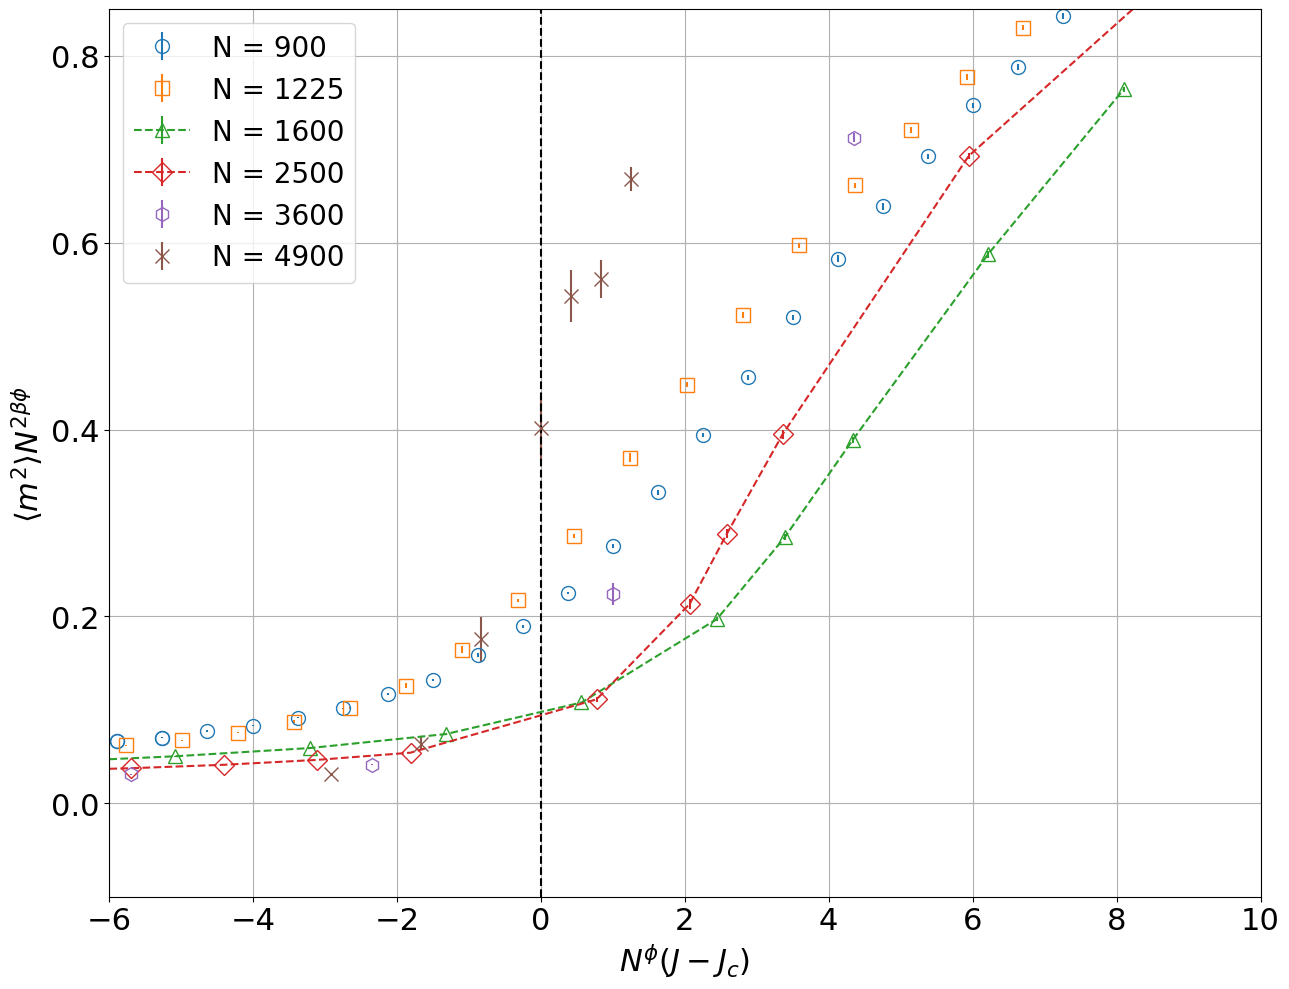
\includegraphics[scale=0.23]{Images/2dmag2scaling1.png}  
%	\caption{$h=0$. Mean radius \eqref{endtoend} and second moment of magnetization \eqref{secondmomentmagnetization} scalings. For left plots we use value $J_{\theta}=1.294$ and for right plots $J_{theta}=1.307$. We assume $\phi=5/7$. }
%	\label{fig:radiusscaling}
%\end{figure}



\subsection{Transition} \label{section:Transition}
To focus on studying phase transition, we calculate two characteristics. The first one is the mean square end-to-end distance scaled using the factor $\nu = \frac{4}{7}$ in \eqref{r_scale}. The second one is Binder cumulant of magnetization \eqref{binderqum}. Figure \ref{fig:bcshort}  presents obtained calculations. 

 \begin{figure}[H]
 	\centering
 	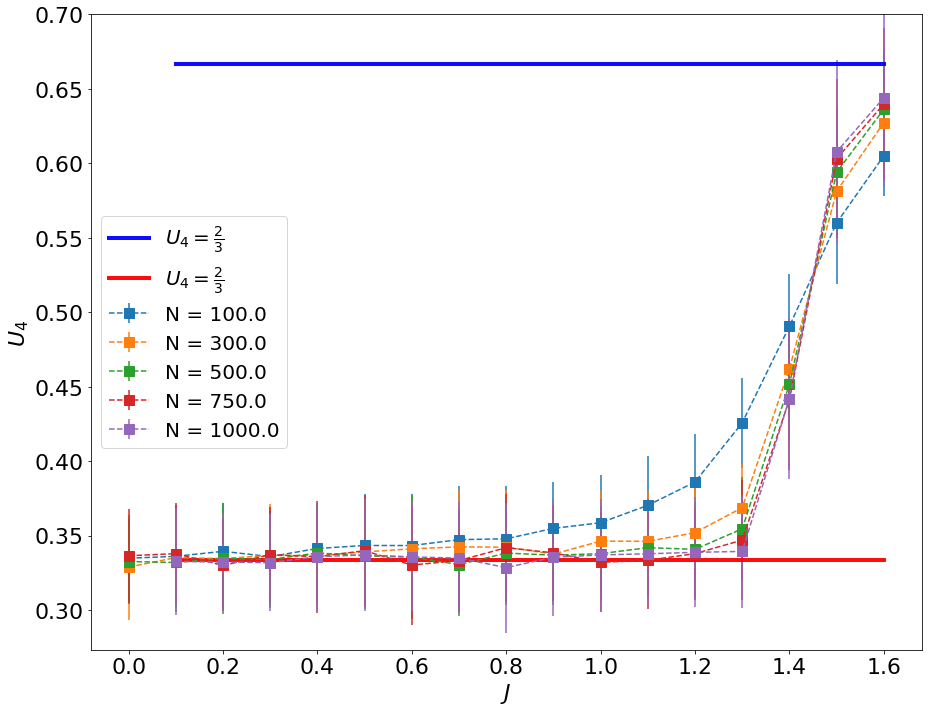
\includegraphics[scale=0.23]{Images/bindercumulants_shortchains.png} 	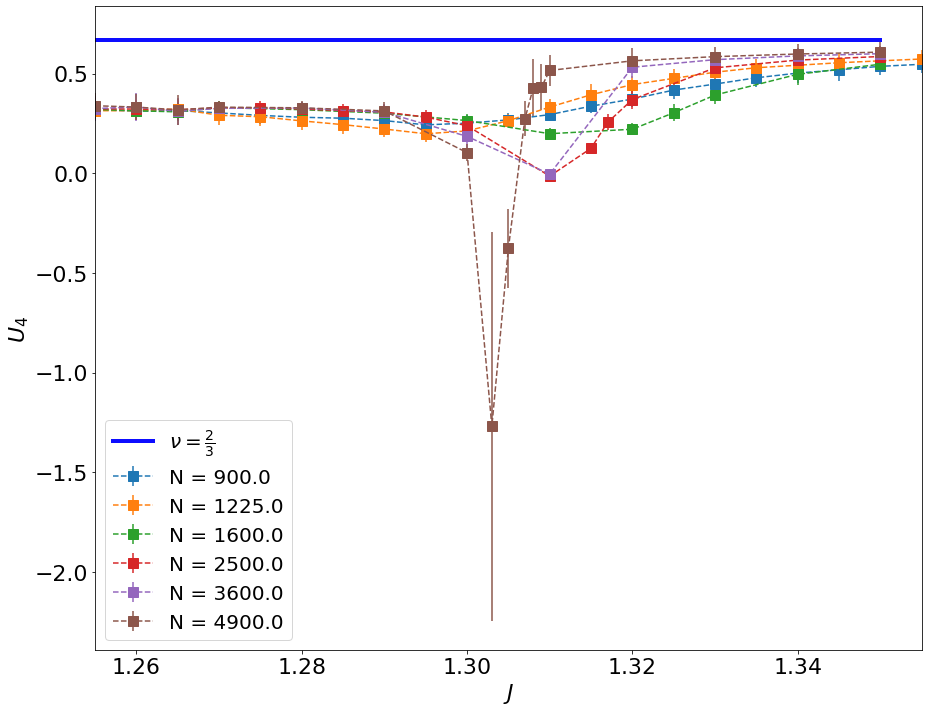
\includegraphics[scale=0.23]{Images/bindercumulants_longchains.png} \\ 
 	 	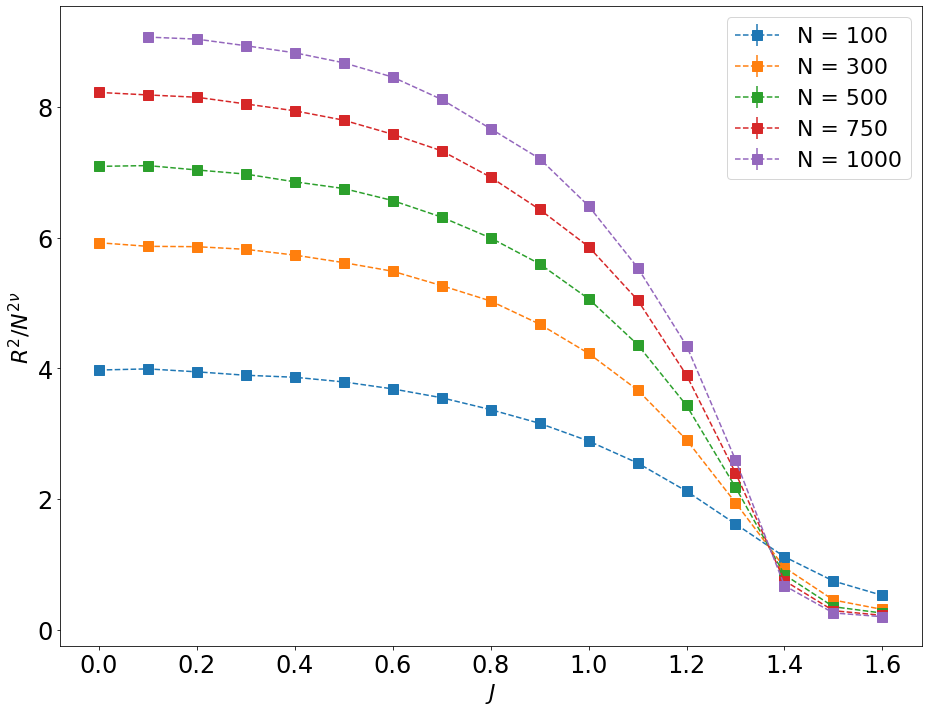
\includegraphics[scale=0.23]{Images/rscaling_shortchains.png}
 	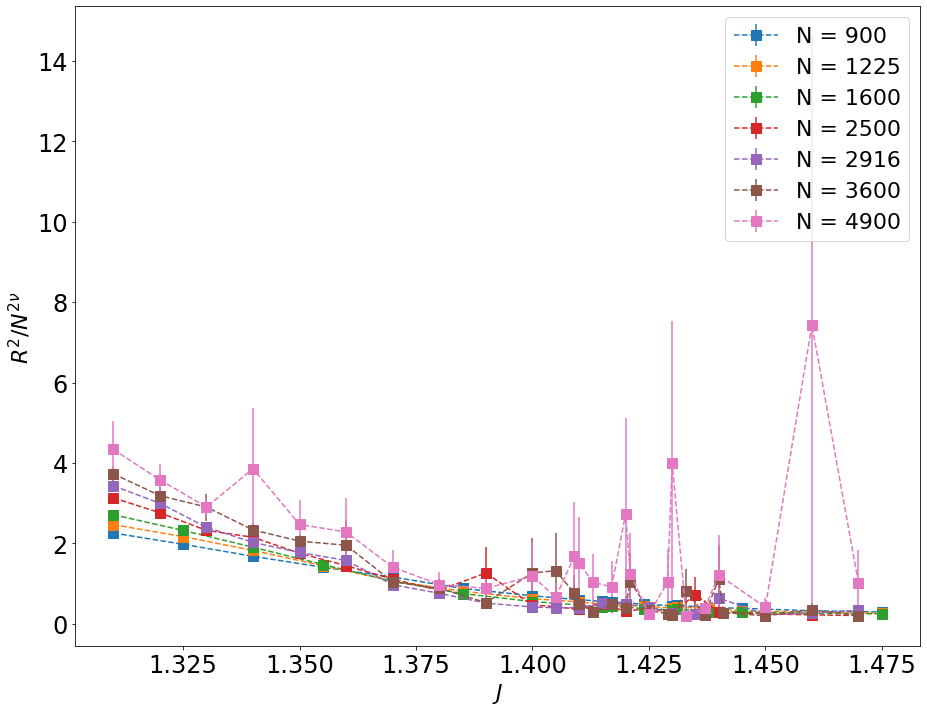
\includegraphics[scale=0.23]{Images/rscaling_longchains.png} 	
 	
 	\caption{$h=0$. Binder  cumulants \eqref{binderqum} and mean radius \eqref{endtoend}.  }
 	\label{fig:bcshort}
 \end{figure}

The Binder parameter  could be used to determine the universality class \cite{binder1981finite}.  At phase transition, the Binder ratio  has a divergent feature at the step if the system has the first order transition. Figure \ref{fig:bcshort}  (top) shows that Binder curves diverge for 2D XY model on SAWs. We can see that in the large systems at the transition region the critical value $ U_4  $ is smaller as $N$ larger. Here, we assume that the model undergoes  the first order transition and study it further using distribution in Section \ref{sec:distributions}. The errorbars for curve $N=4900$ are huge, however, we can narrow the region where the phase transition point is located: $J_{cr} \in [1.29; 1.32]$. 

In the bottom of Figure \ref{fig:bcshort} we can see that scaled curves of mean radius cross approximately at the same point where long chains have minimum values of Binder cumulant. The right plot also shows us the finite size effect. To make estimation of the critical point, we make following procedure with paired crossings using Monte-Carlo data: 

1. Choose the pair of two different N values for length of the chain. Choose the range of values for interaction energy J. This segment should be as short as possible and include the point of intersection of the two curves. 

2. For each point from the set generate $n_{samples}$ values using Normal distribution with mean and standard error of $\langle R^2 \rangle / N^ {2 \nu}$ as parameters: $ X_{J, N} \sim N (\langle R^2 \rangle / N^ {2 \nu}, \sigma (\langle R^2 \rangle / N^ {2 \nu}))$. We generate for each value $J$ and $N$ 100 samples: $n_{samples} = 100$. 

3. Using generated set, for each pair $J$ and $N$ make estimation for mean and standard deviation $\langle  R^2 / N^ {2 \nu} (J, N)\rangle$.

4. Apply weighted least squares regression to find crossing point. Save the obtained estimation for $\hat{J_{\theta}}$. 

5. Repeat steps 2-5 $n_{lines}$ times. We repeat it $n_{lines}=1000$ times. 

6. At the end, we have $n_{lines}$ of estimated $\hat{J_{\theta}}$ where two curves cross. This set of obtained estimations is histogram in Figure \ref{fig:Jthetahistogram}. 

 \begin{figure}
	\centering
	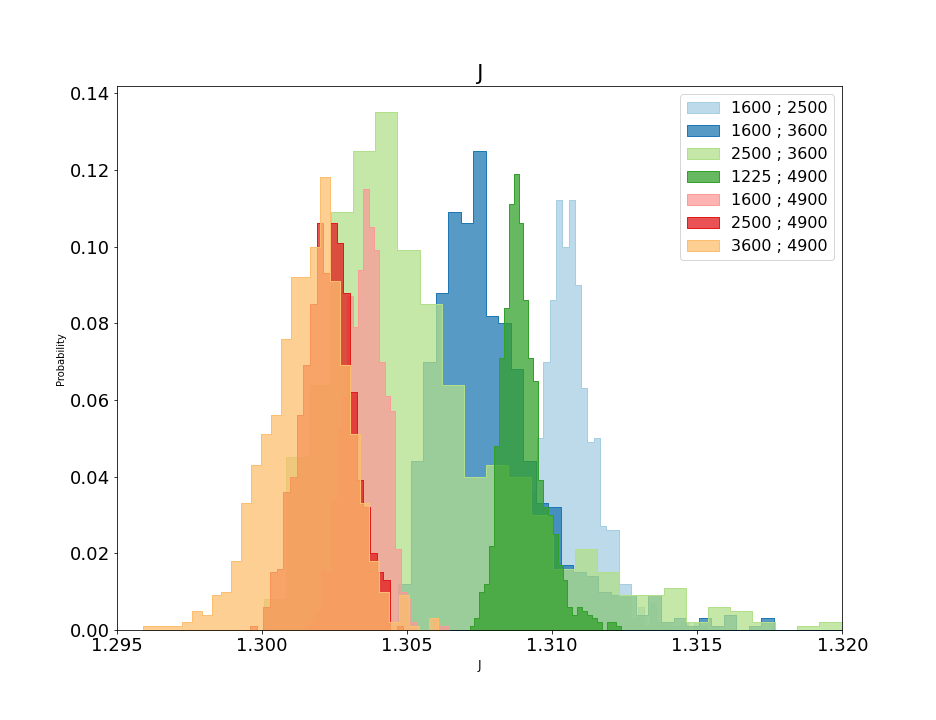
\includegraphics[scale=0.28]{Images/radius_hist_cov.png}
	\caption{$h=0$. Histograms of estimated $J_{\theta}$ from paired regressions.  }
	\label{fig:Jthetahistogram}
\end{figure}

Histograms for pairs from Figure \ref{fig:Jthetahistogram} shows us how the size of systems affect the estimations $\hat{J_{\theta}}$. One way to choose the estimation for phase transition point $\hat{J_{\theta}}$ in thermodynamic limit is to focus on pairs for long chains such as $N=3600$ and $N=4900$. Consider the set of results for $N=4900$. We have calculations for four pairs $[N_i, 4900]$ which presented in Figure \ref{fig:Jthetahistogram}. We construct the dependence of estimates $\hat{J_{\theta}}$ on $1/N_i$. Using this measurements, we perform curve-fitting using weighted least squares regression. The fitting results are plotted in Figure \ref{fig:JthetaLinear}. Estimation of criticl point is the point of the limit $1/N_i \rightarrow 0$. We obtain the following results: 
\begin{equation}
\label{eq:critical_J_theta_2D}
J_{\theta}^{3600} \approx 1.3(06); J_{\theta}^{4900} \approx 1.3(04).
\end{equation}
%Estimated value from the zero point: $J_{\theta} \approx 1.3(0)$.

 \begin{figure}[H]
	\centering
	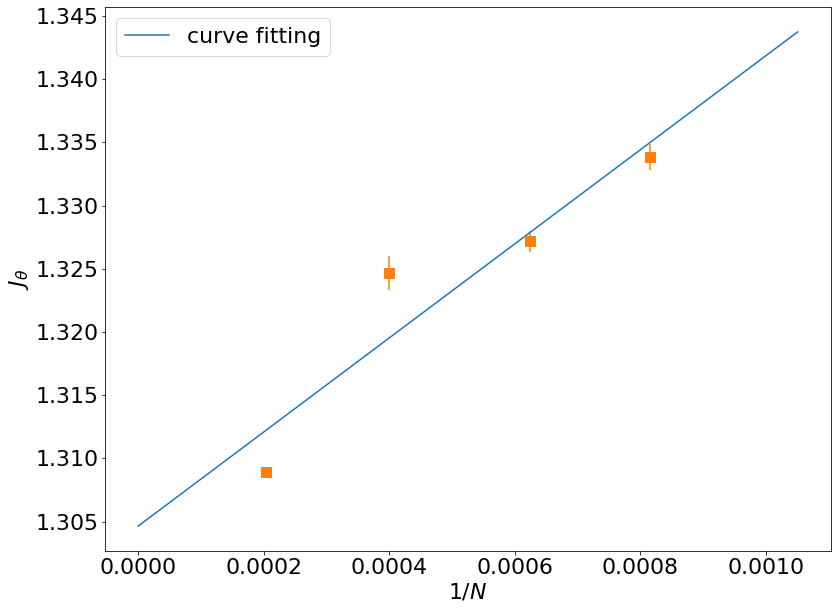
\includegraphics[scale=0.2]{Images/criticalr2_3600.png}
	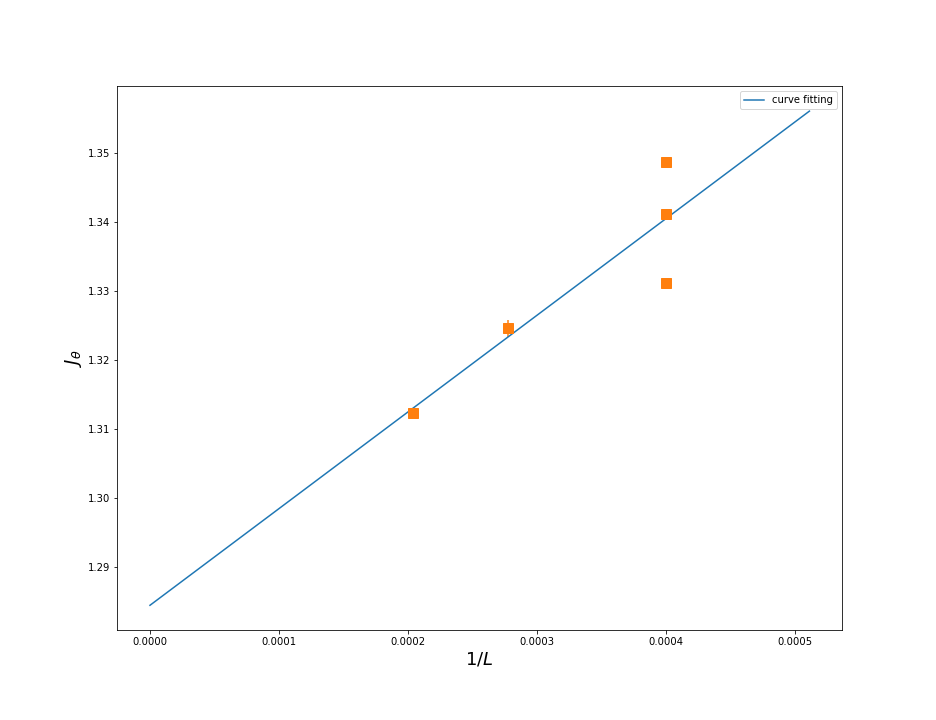
\includegraphics[scale=0.2]{Images/criticalr2.png}
	\caption{$h=0$. Pairs with $N=3600$ (left) and $N=4900$ (right).  }
	\label{fig:JthetaLinear}
\end{figure}
 



\subsection{Distribution of $\langle cos \theta \rangle$ and $\langle e \rangle$ } \label{sec:distributions}
To study the phase transition order, we look to distributions of energy and magnetization.

We start our observation of distributions with quite shore chain $N=1600$. Here (Figure \ref{fig:distributions}, top), we notice that energy distribution shape is getting wider around the critical region $J_{cr} \in [1.29; 1.32]$ which was defined using results from Figure \ref{fig:bcshort}. These curves  do not help enough to determine signs of first order transition. 

Next, we turn our attention to the longer chains $N=2500$ (Figure \ref{fig:distributions}, medium). In this case, we see broad maybe-bimodal shape of energy distribution at the points $J=1.317$ and $J=1.32$.  

Finally, we investigate the Monte-Carlo results for $N=4900$ (Figure \ref{fig:distributions}, bottom). The curve of the energy distribution obtained for simulation in $J=1.307$ is bimodal which corresponds to the first-order phase transition.   

  \begin{figure}[H]
 	\centering
 	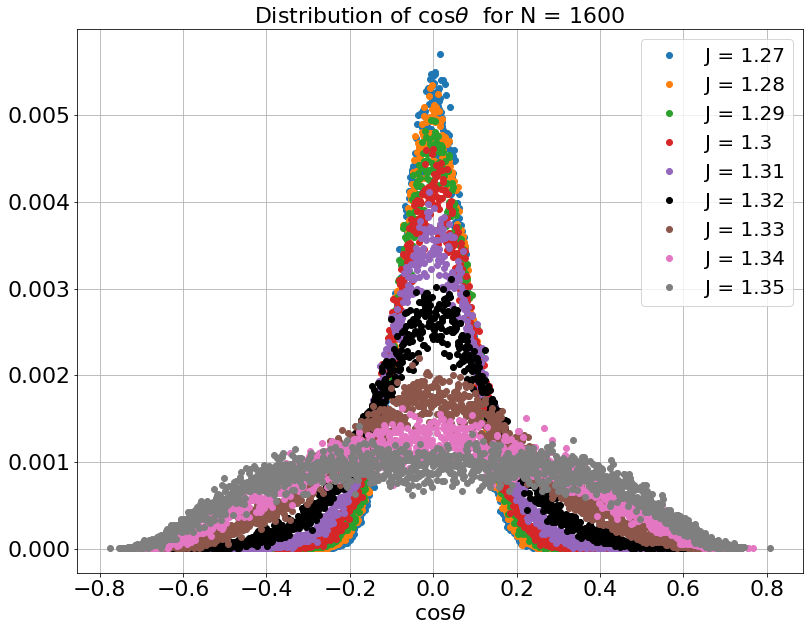
\includegraphics[scale=0.25]{Images/distr_cos_1600.png}
 	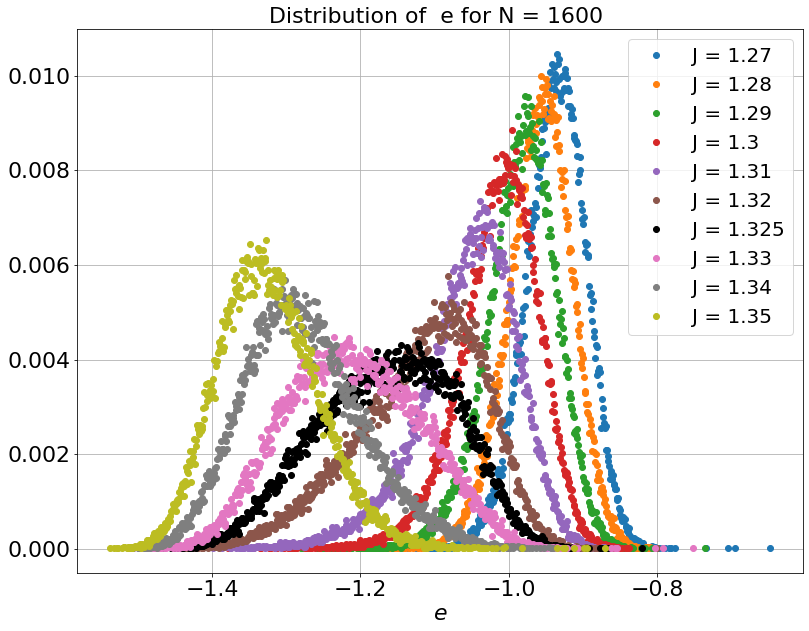
\includegraphics[scale=0.25]{Images/distr_energy_1600.png} \\
 	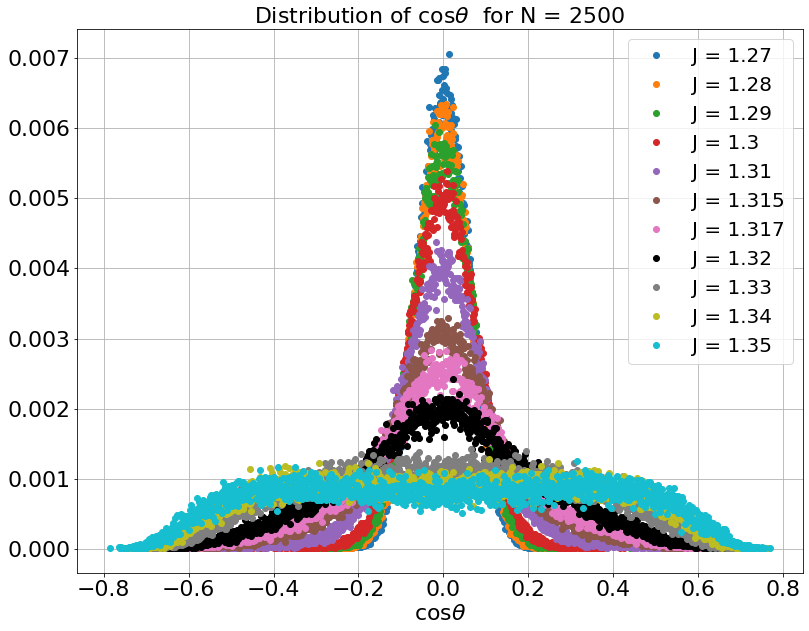
\includegraphics[scale=0.25]{Images/distr_cos_2500.png}
 	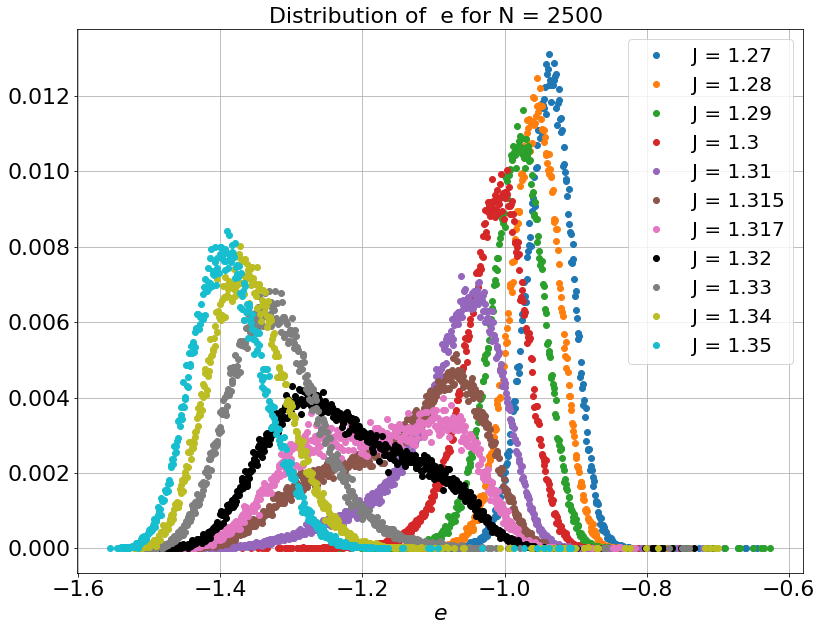
\includegraphics[scale=0.25]{Images/distr_energy_2500.png}
 	\\
 	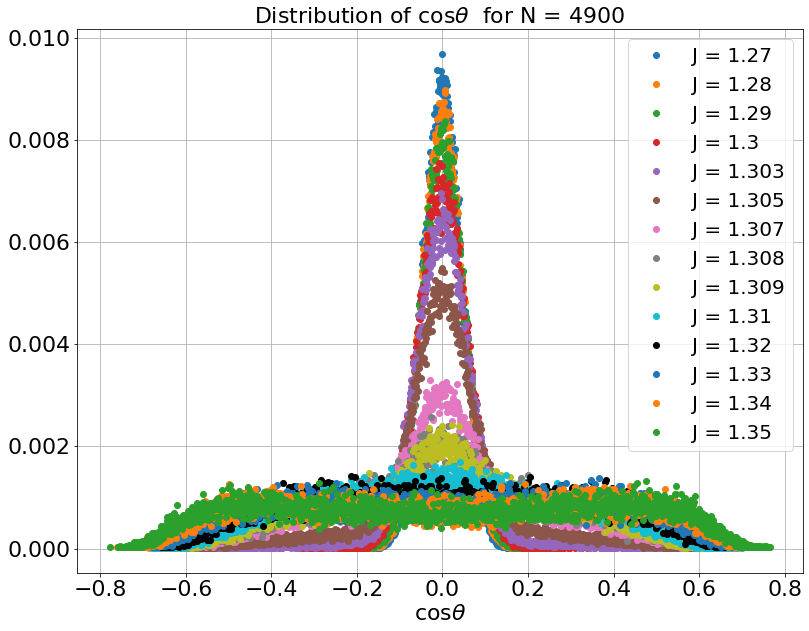
\includegraphics[scale=0.25]{Images/distr_cos_4900.png}
 	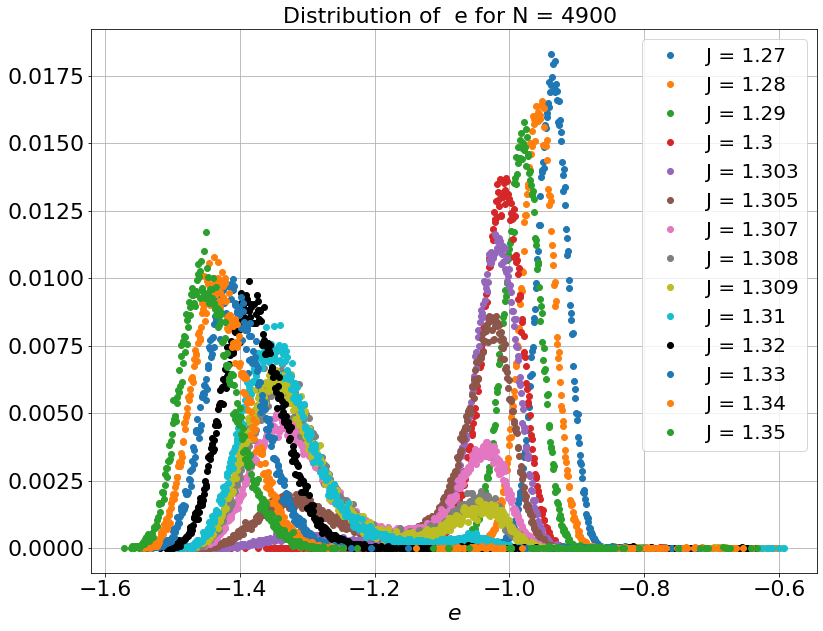
\includegraphics[scale=0.25]{Images/distr_energy_4900.png}
 	\caption{$h=0$.  }
 	\label{fig:distributions}
 \end{figure}

To examine that shape of the energy critical distribution is truly bimodal, we monitor the curve over simulation and fix four phase of the simulation in Figure \ref{fig:distributione4900}. We see that the results at the beginning are quite noisy, however, the data converge to bimodal shape. Here, we can make an estimation $J_{\theta} \approx 1.3(0)$ as we obtain bimodal plot at the point $J=1.307$. 


 \begin{figure}[H]
	\centering
	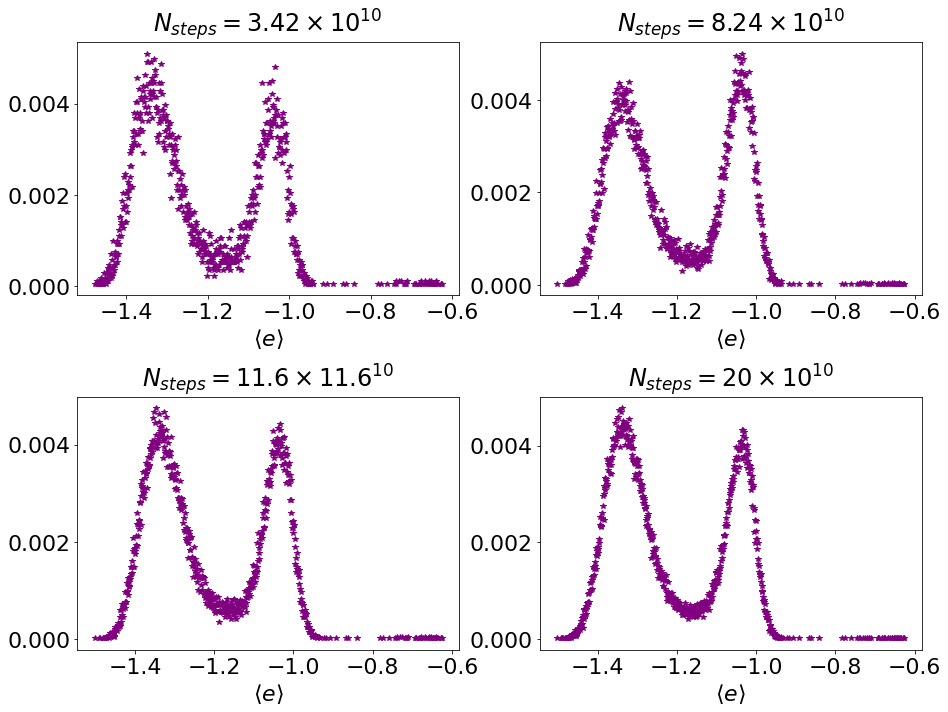
\includegraphics[scale=0.36]{Images/distr_energy_4900_time.png}
	\caption{$h=0$.  }
	\label{fig:distributione4900}
\end{figure}

We also observe the distributions of $\langle cos \theta \rangle$ as a magnetic property. We notice that over the critical region the shapes of distributions are far from Normal-like curves and have signs of phase coexistence. \textbf{foster ?}

 \begin{figure}[H]
	\centering
	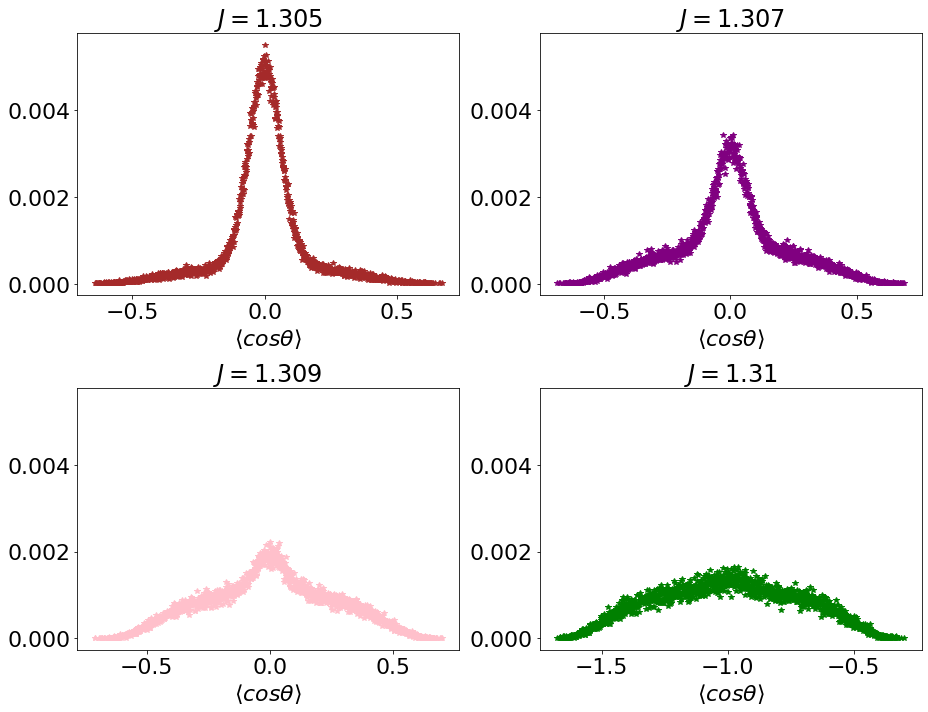
\includegraphics[scale=0.36]{Images/distr_cos_4900_J.png}
	\caption{$h=0$.  }
	\label{fig:distributioncos4900}
\end{figure}


\subsection{Summary for 2D case}
We study XY model on self-avoiding walks on the square lattice (2D case) using Monte-Carlo simulations. In this work, we consider regime when both conformations and spins are dynamic. Our computational results are consistent with assumption that such model has first-order transition at the critical point. 





\section{XY model on SAWs, 3D}


\subsection{Thermodynamic properties}

 \begin{figure}[t]
	\centering
	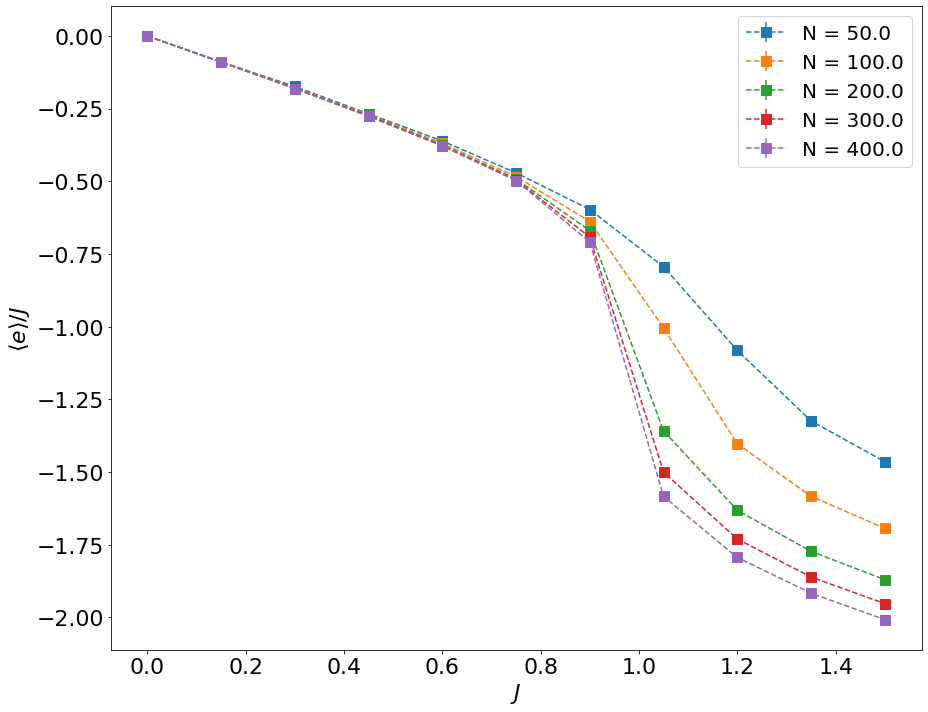
\includegraphics[scale=0.23]{Images/3_energy_shortchains.png}
	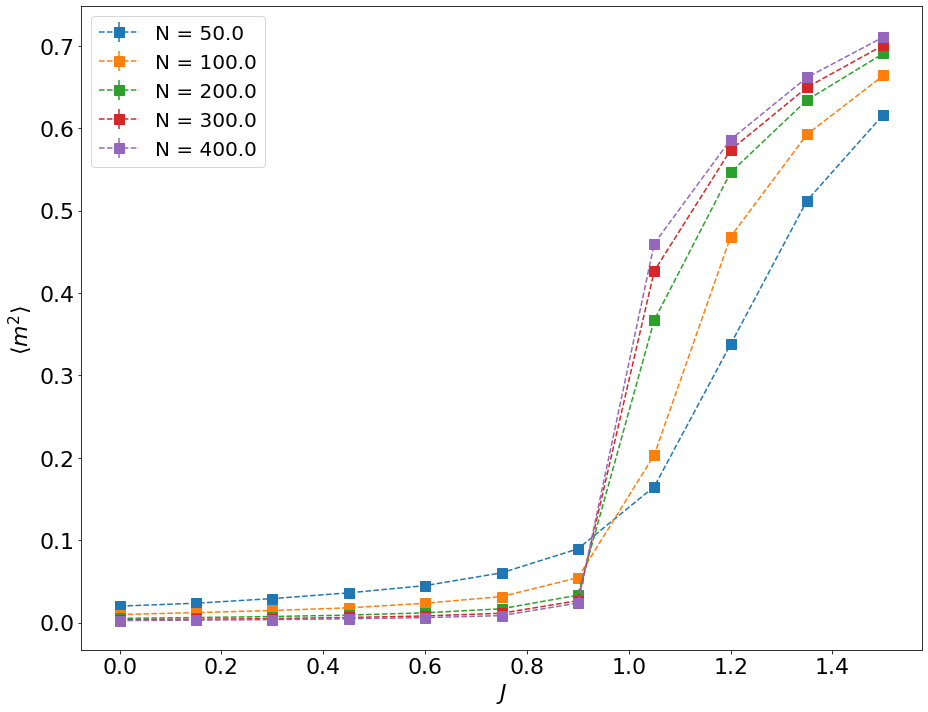
\includegraphics[scale=0.23]{Images/3_magnetization2_shortchains.png} \\
	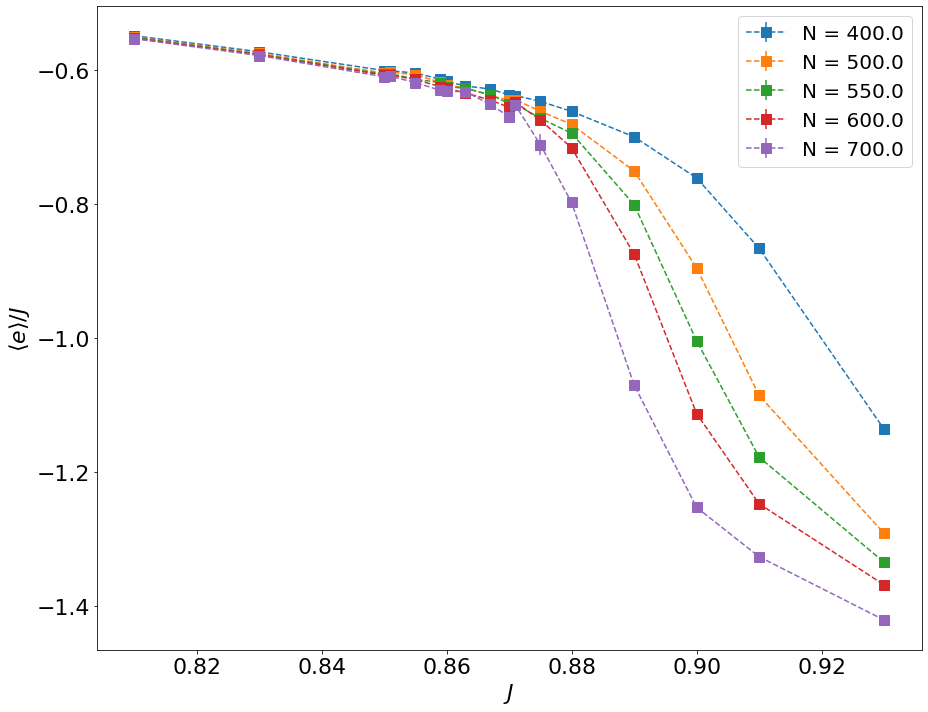
\includegraphics[scale=0.23]{Images/3_energy_longchains.png}
	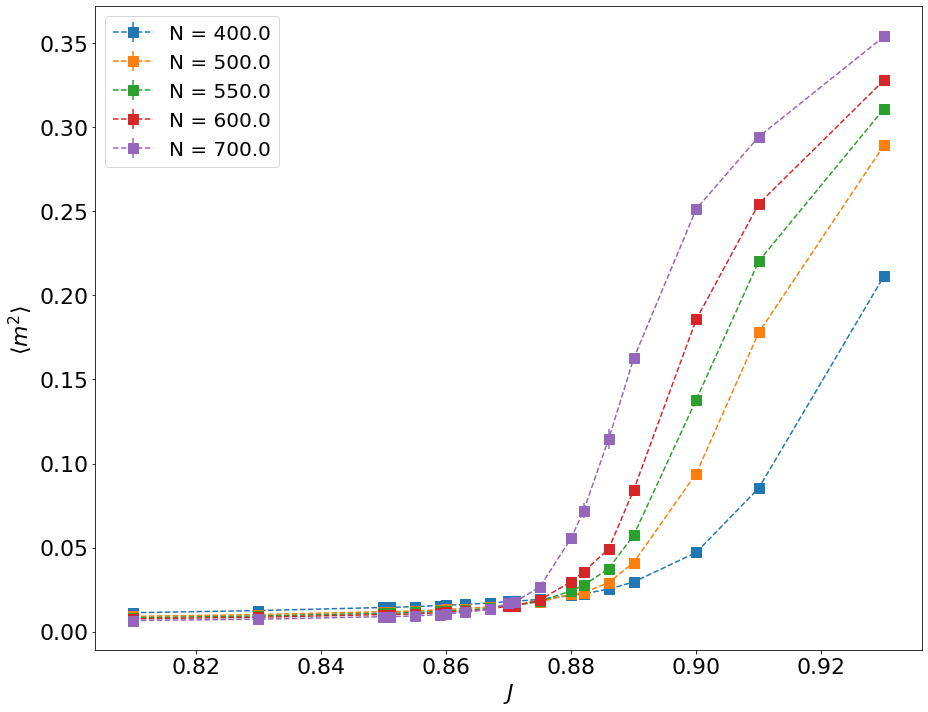
\includegraphics[scale=0.23]{Images/3_magnetization2_longchains.png}
	\caption{$h=0$. Mean energy \eqref{hamiltonian} and   second moment of magnetization \eqref{secondmomentmagnetization}. }
	\label{fig:energymagshort_3D}
\end{figure}


\subsection{Structural properties}


 \begin{figure}[H]
	\centering
	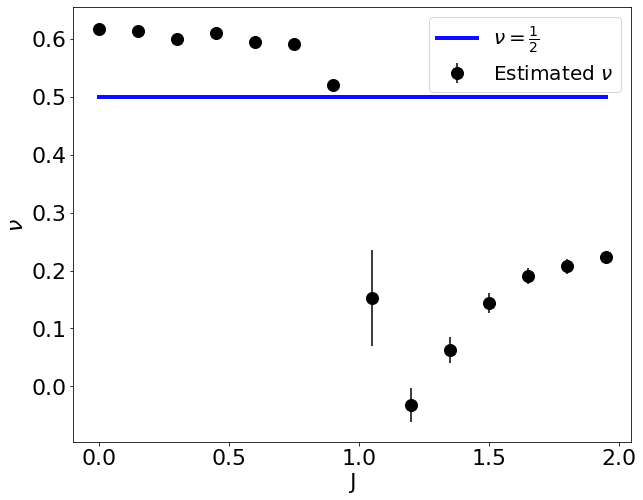
\includegraphics[scale=0.36]{Images/3_nu_shortchains.png}
	\caption{$h=0$. Estimations with errorbars of critical exponent $\nu$ .   }
	\label{fig:nushort3D}
\end{figure}



\subsection{Transition}

 \begin{figure}[H]
	\centering
	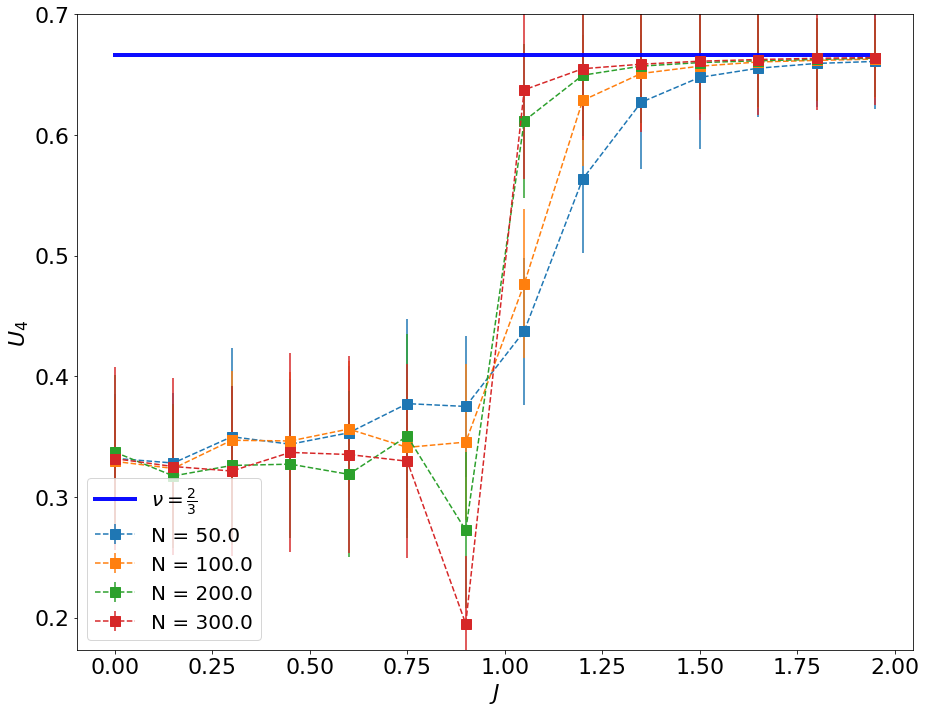
\includegraphics[scale=0.23]{Images/3_bindercumulants_shortchains.png} 	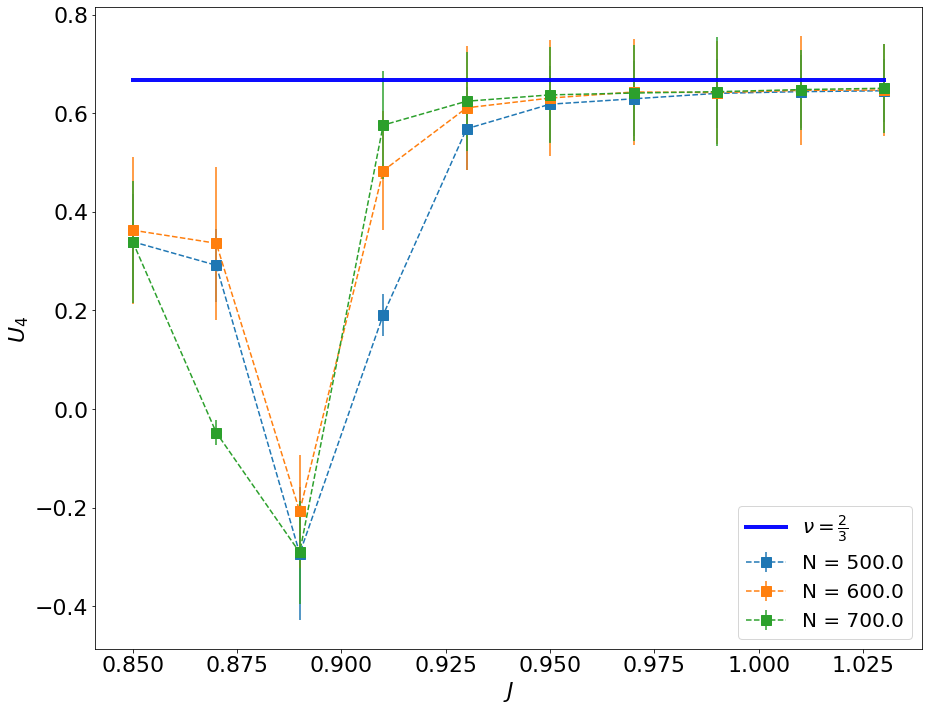
\includegraphics[scale=0.23]{Images/3_bindercumulants_longchains.png} \\ 
	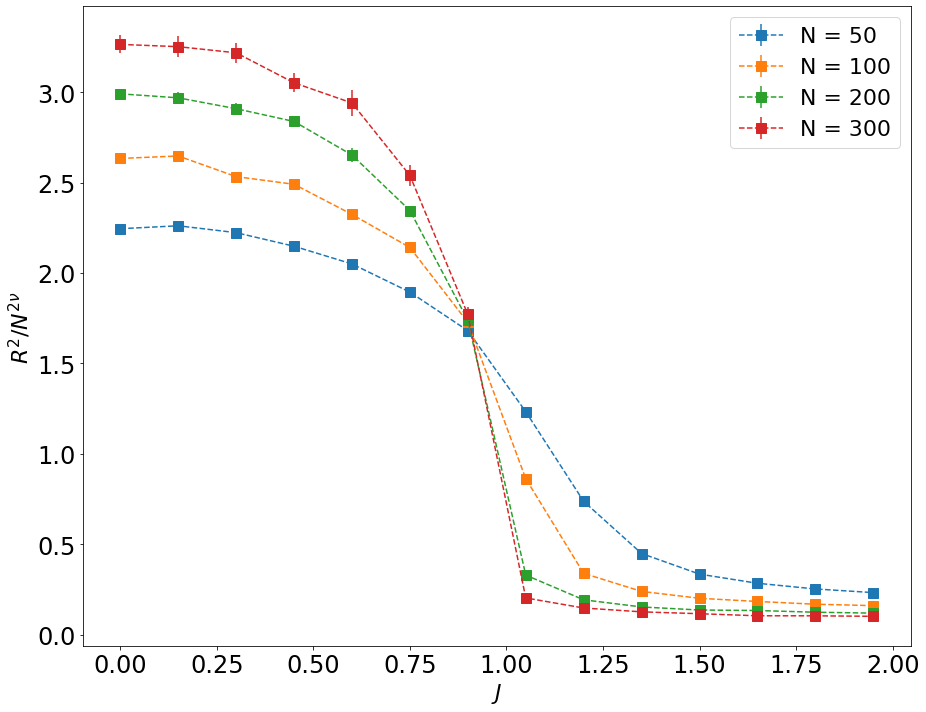
\includegraphics[scale=0.23]{Images/3_rscaling_shortchains.png}
	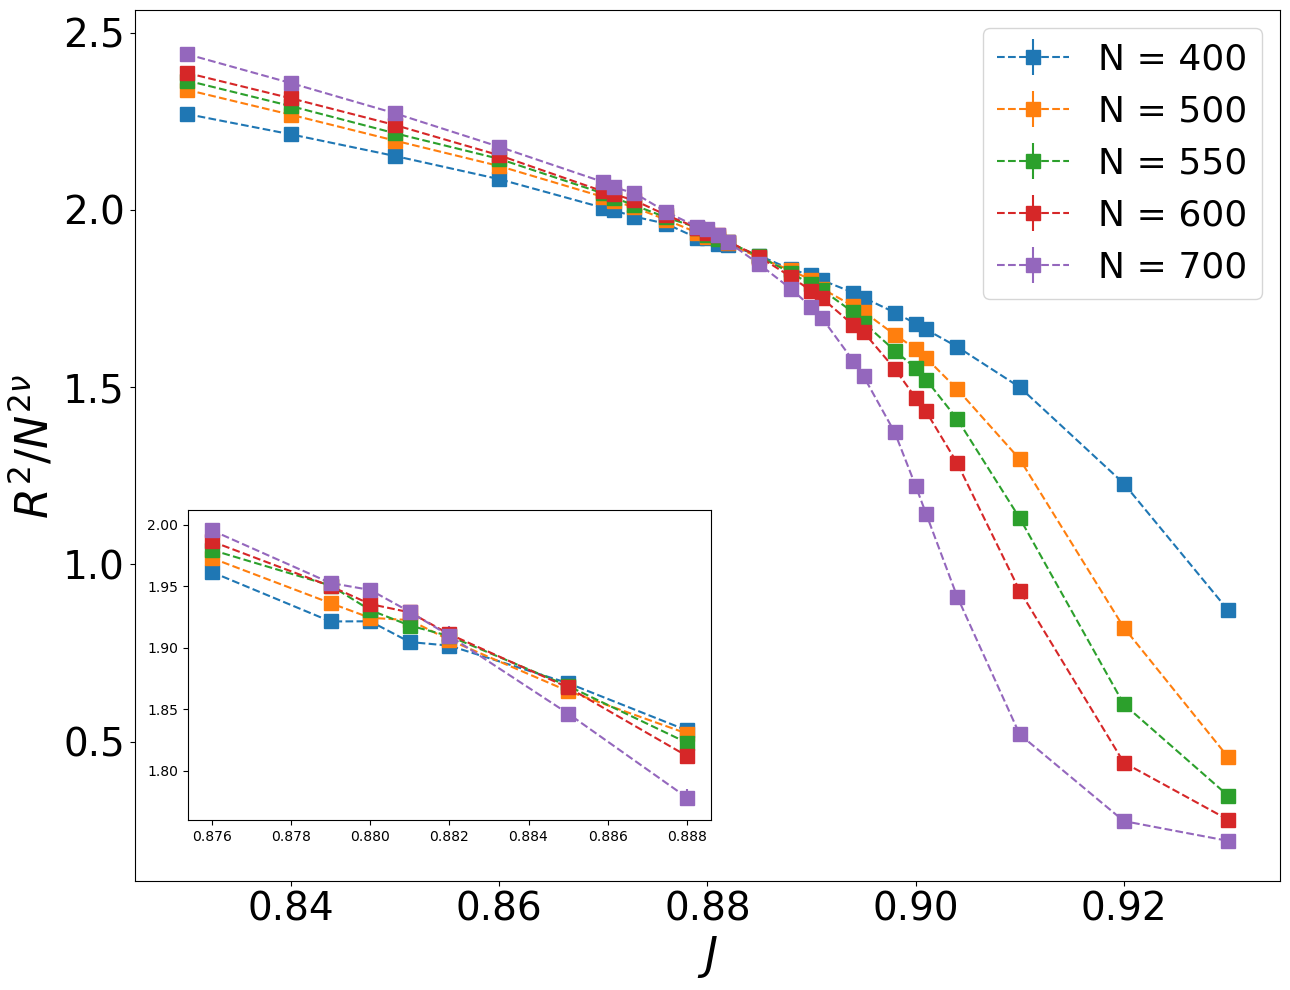
\includegraphics[scale=0.23]{Images/3_rscaling_longchains.png} 	
	
	\caption{$h=0$. Binder  cumulants \eqref{binderqum} and mean radius \eqref{endtoend}.  }
	\label{fig:bcshort_3D}
\end{figure}



\subsection{Distribution of $\langle cos \theta \rangle$ and $\langle e \rangle$ } \label{sec:distributions_3D}



  \begin{figure}[H]
	\centering
	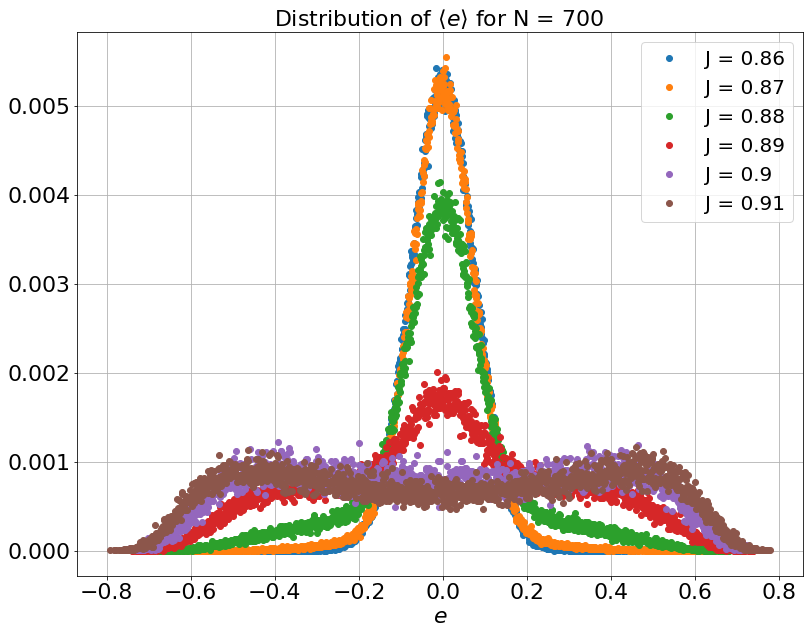
\includegraphics[scale=0.25]{Images/distr_cos_700.png}
	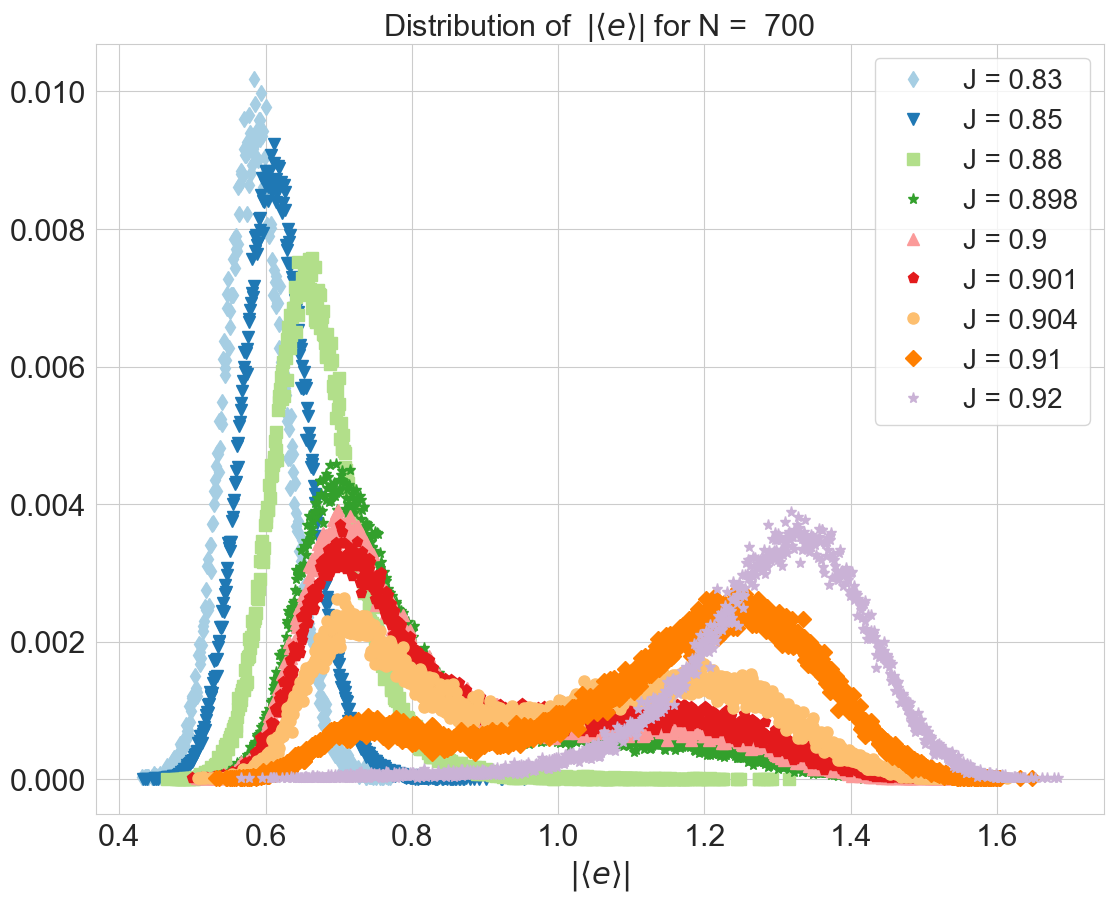
\includegraphics[scale=0.25]{Images/distr_energy_700.png}
	\caption{$h=0$.  }
	\label{fig:distributions_3D}
\end{figure}